\begin{atiTask}[
  title = Rotation und Divergenz
  %call = Zusatzaufgabe,
]

Konstruieren Sie jeweils ein Vektorfeld, das die folgenden Bedingungen erfüllt, und machen Sie eine Probe. Dabei ist 
\[\divergence \vec{F} = \leibnizPartialDerivative{F_x}{x}+\leibnizPartialDerivative{F_y}{y}+\leibnizPartialDerivative{F_z}{z}\]
\begin{atiSubtasks}
\item $\curl \vec{v}$ besitzt nur eine von $x$-abhängige Komponente in $\vectorZ$-Richtung. $\divergence \vec{v}$ verschwindet nicht.
\item $\divergence \vec{w}$ hängt nur von $x^2+y^2$ ab. $\curl \vec{w}$ hat keine verschwindende Komponente.
\end{atiSubtasks}
\end{atiTask}

\begin{atiSolution}
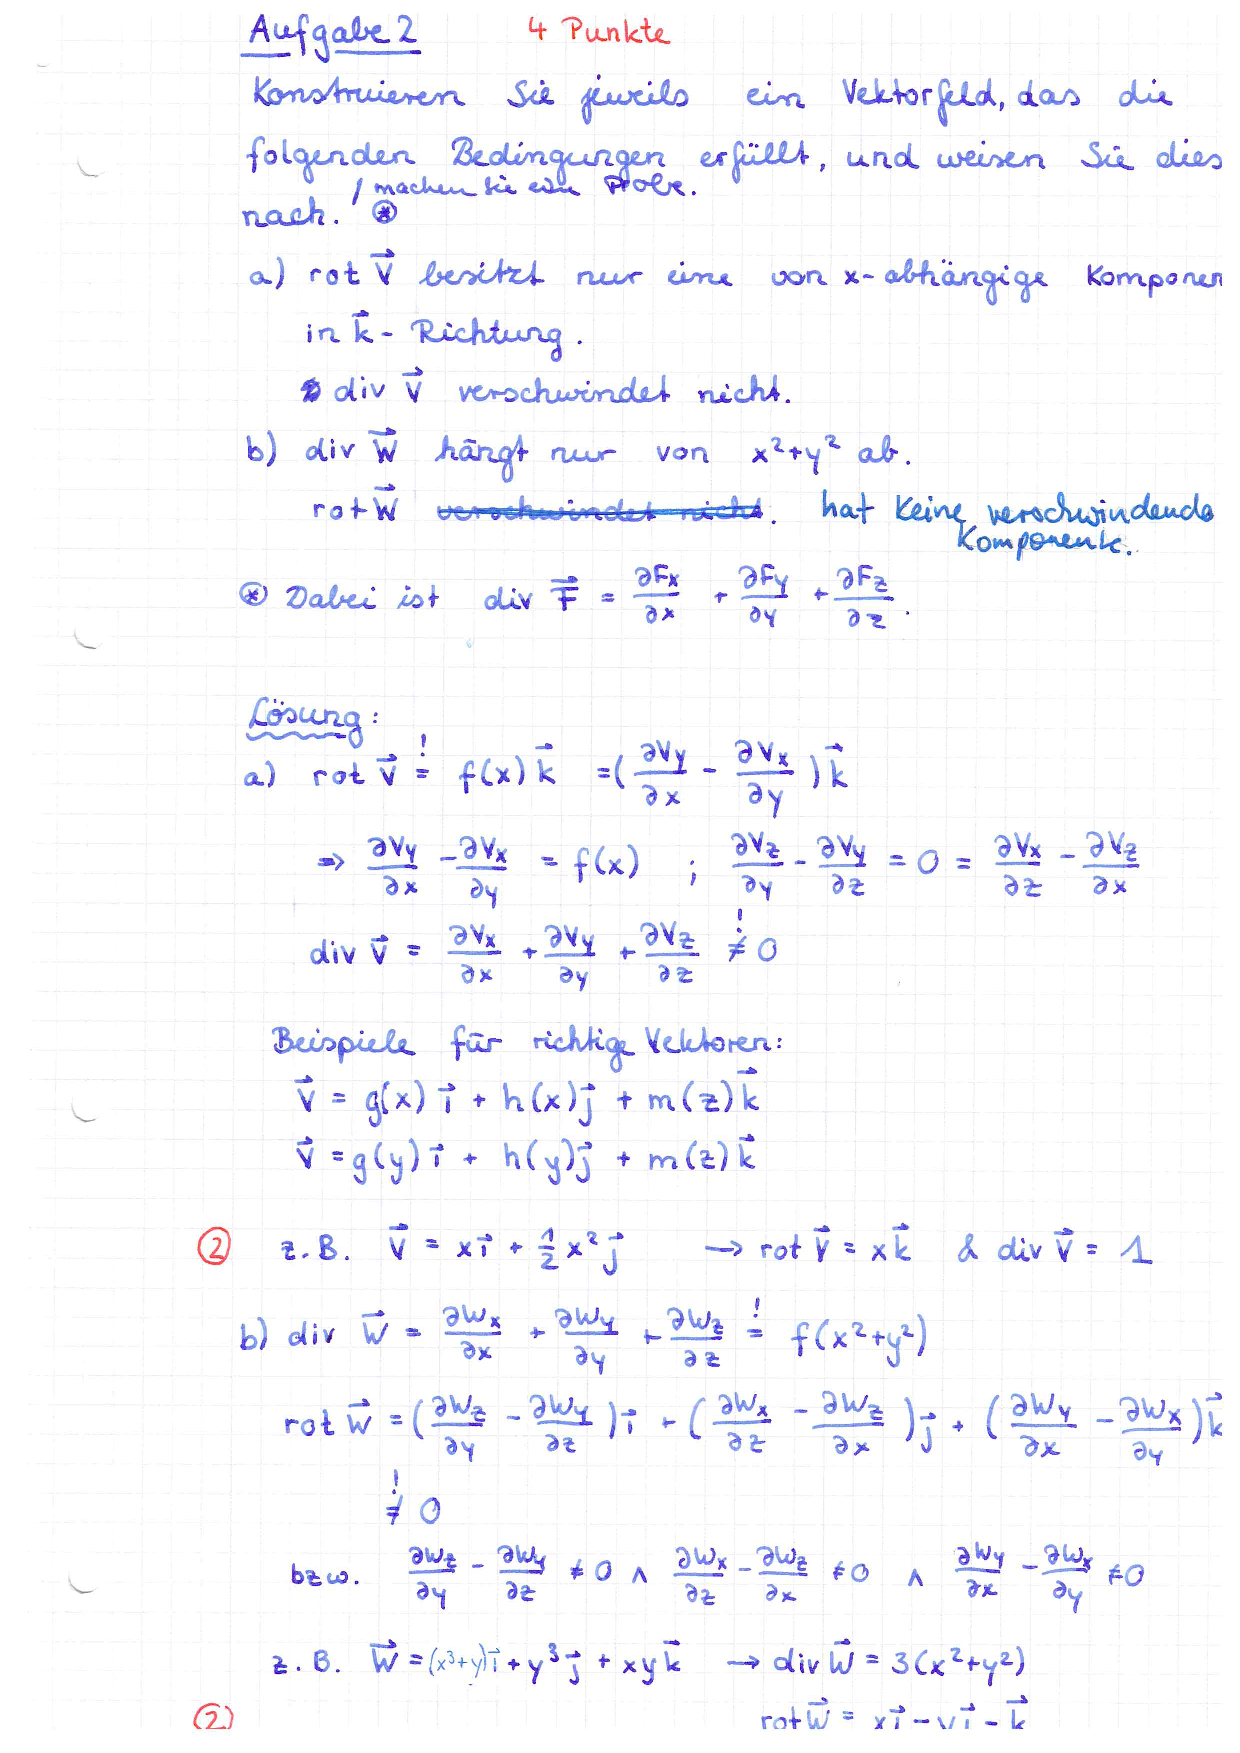
\includepdf[pages=-]{solution-rotation_iii.pdf}
%\begin{atiSubtasks}
%\item $\curl \vec{v}\overset{!}{=}f(x)\vectorX =\left(\leibnizPartialDerivative{v_y}{x}-\leibnizPartialDerivative{v_x}{y}\right)\vectorZ$
%$\Rightarrow \leibnizPartialDerivative{v_y}{x}-\leibnizPartialDerivative{v_x}{y}=f(x)$, 
%Beispiele für richtige Vektoren:
%$\vec{v}=g(x)\vectorX+h(x)\vectorY+m(z)\vectorZ$\\
%$\vec{v}=g(y)\vectorX+h(y)\vectorY+m(z)\vectorZ$
%z.B. $\vec{v}=x\vectorX+1/2x^2\vectorY\rightarrow \curl \vec{v}=x\vec{k}$ und $\divergence \vec{v}=1$
%\end{atiSubtasks}
%
\end{atiSolution}